\chapter{\ifproject%
\ifcpe โครงสร้างและขั้นตอนการทำงาน\else Project Structure and Methodology\fi
\else%
\ifcpe โครงสร้างของโครงงาน\else Project Structure\fi
\fi
}


\makeatletter

% \renewcommand\section{\@startsection {section}{1}{\z@}%
%                                    {13.5ex \@plus -1ex \@minus -.2ex}%
%                                    {2.3ex \@plus.2ex}%
%                                    {\normalfont\large\bfseries}}

\makeatother
%\vspace{2ex}
% \titleformat{\section}{\normalfont\bfseries}{\thesection}{1em}{}
% \titlespacing*{\section}{0pt}{10ex}{0pt}
ในบทนี้จะกล่าวถึงผลสรุปจากการสํารวจความคิดเห็นของนักศึกษาเกี่ยวกับตารางสอบปลายภาค ข้อมูลที่จำเป็นต้องใช้สำหรับการพัฒนาโปรแกรม รวมถึงโครงสร้างข้อมูลรับเข้าและข้อมูลส่งออกของโปรแกรม
ซึ่งจากความต้องการพัฒนาระบบจัดตารางสอบปลายภาคเพื่อให้นักศึกษามีอิสระในการเลือกลงทะเบียนเรียนมากขึ้นดังที่กล่าวในตอนที่ \ref{sec:project_rationale} เราจึงต้องการทราบความคิดเห็นของนักศึกษาในมหาวิทยาลัยเชียงใหม่เกี่ยวกับตารางสอบปลายภาค 
ทำให้เราได้จัดทำแบบสอบถามขึ้นเพื่อสอบถามความคิดเห็นของนักศึกษามหาวิทยาลัยเชียงใหม่ ทั้งนักศึกษาปัจจุบันและนักศึกษาเก่าที่สำเร็จการศึกษาแล้ว ว่ามีความคิดเห็นอย่างไรกับตารางสอบปลายภาคในปัจจุบัน และหากเลือกได้อยากจะสอบในช่วงเวลาใดบ้าง ๆ ในตารางเวลาของสัปดาห์ที่จัดสอบ 
โดยจะพยายามนำข้อมูลที่ได้มาใช้ในการอ้างอิงเพื่อออกแบบอัลกอลิทึมสำหรับประมวลผลหาวิธีการจัดตารางสอบที่เหมาะสมที่สุดที่เป็นไปได้สำหรับนักศึกษาทุกคน
\TSNAreply{เพิ่มตรงนี้แล้วครับ}

\section{การสำรวจความคิดเห็นของนักศึกษาเกี่ยวกับตารางสอบปลายภาค}
\CIreply{เพิ่มรายละเอียดว่าผู้ตอบแบบสอบถามมาจากคณะใดบ้าง ชั้นปี ฯลฯ}
จากผลสำรวจของแบบสอบถามเกี่ยวกับตารางสอบปลายภาคของมหาวิทยาลัยชียงใหม่ โดยขอความร่วมมือนักศึกษาในมหาวิทยาลัย
ทั้งนักศึกษาที่กำลังศึกษาอยู่และทั้งที่สำเร็จการศึกษาไปแล้ว เพื่อให้ช่วยตอบแบบสอบถามความคิดเห็นเกี่ยวกับ ข้อดี ข้อเสีย ความพึงพอใจในตารางสอบของตนเอง
รวมถึงปัญหาเกี่ยวกับตารางสอบปลายภาคที่เคยพบหรือได้รับผลกระทบโดยตรง โดยจากผลการสำรวจกลุ่มสำรวจจำนวน 95 คน พบว่าผู้ตอบแบบสอบถามส่วนใหญ่นั้นตรวจสอบตารางสอบของทุกวิชาที่ต้องการจะลงทะเบียน
ก่อนที่จะลงทะเบียนเรียนอย่างสม่ำเสมอ แต่ยังมีผู้ตอบแบบสอบถามบางส่วนนั้นที่ตรวจสอบตารางสอบเพียงบางวิชาก่อนจะลงทะเบียนเรียน และยังมีมีผู้ตอบแบบสอบถามส่วนน้อยที่ตอบว่าไม่เคยตรวจสอบตารางสอบของตนเองเลย ดังกราฟที่ \ref{fig:check_before_enrollment}
\begin{figure}
  \begin{center}
    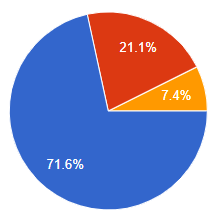
\includegraphics{images/checking_schedule_before_enrollment.png}\\[2ex]
    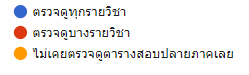
\includegraphics{images/legend_for_checking_schedule_before_enrollment.png}
  \end{center}
  \caption[Poem]{จำนวนผู้ตอบแบบสอบถามที่ตรวจสอบตารางสอบปลายภาคก่อนการลงทะเบียน}
  \label{fig:check_before_enrollment}     
\end{figure}
จากผลการสำรวจเรายังพบว่ากลุ่มสำรวจกว่า 80\% ไม่ทราบว่าสำนักทะเบียนมหาลัยเชียงใหม่ จัดตารางสอบปลายภาคอย่างไร ดังแสดงในกราฟที่ \ref{fig:registration_exam}
\begin{figure}
  \begin{center}
    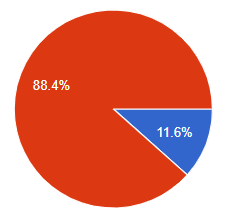
\includegraphics{images/registration_exam.png}\\[2ex]
    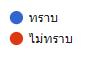
\includegraphics{images/legend_for_registration_exam.png}
  \end{center}
  \caption[Poem]{จำนวนผู้ตอบแบบสอบถามที่ทราบวิธีการจัดตารางสอบปลายภาคของสำนักทะเบียน}
  \label{fig:registration_exam}     
\end{figure}
จากผลการสำรวจเรายังสามารถสรุปผลได้ดังนี้
วันที่ผู้ทำแบบสอบถามต้องการจะสอบมากที่สุด 7 อันดับแรก โดยเรียงลำดับจากมากไปน้อย
\begin{enumerate}
  \item สัปดาห์ที่หนึ่ง วันจันทร์
  \item สัปดาห์ที่หนึ่ง วันพุธ
  \item สัปดาห์ที่หนึ่ง วันศุกร์ 
  \item สัปดาห์ที่หนึ่ง วันอาทิตย์
  \item สัปดาห์ที่สอง วันอังคาร
  \item สัปดาห์ที่สอง วันพฤหัสบดี
  \item สัปดาห์ที่สอง วันเสาร์
\end{enumerate}

\noindent จากข้อมูลเราสามารถบอกได้ว่าเวลาที่ผู้ทำแบบสอบถามส่วนใหญ่ต้องการที่จะสอบในแต่ละวันคือ
ช่วงเวลา 12.00-15.00น. ซึ่งผู้ทำแบบสอบถามส่วนมากต้องการจะสอบช่วงเวลานี้มากกว่า 15.30-18.00น. และ 08.00-11.00น. ตามลำดับ ดังกราฟ \ref{fig:time}
\begin{figure}
  \begin{center}
    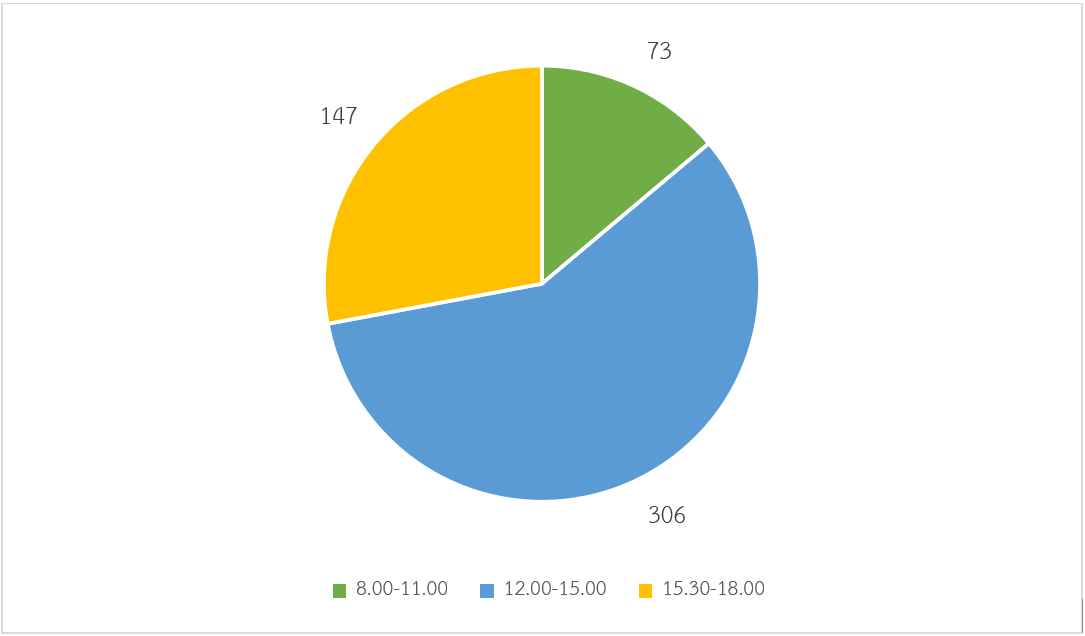
\includegraphics[width=\linewidth]{images/pie_chart_for_final_exam_time.png}
  \end{center}
  \caption[Poem]{ความต้องการในสอบของผู้ตอบแบบสอบถามในแต่ละเวลา}
  \label{fig:time}     
\end{figure}
และถ้าเราทำการรวมช่วงเวลาที่ผู้ตอบแบบสอบถามต้องการสอบกับวันที่ผู้ตอบแบบสอบถามต้องการสอบเข้าด้วยกันดังกราฟที่ \ref{fig:time_slot} จะสามารถสรุปวันที่ผู้ทำแบบสอบถามต้องการจะสอบมากที่สุด 7 อันดับแรก โดยสามารถเรียงลำดับจากมากไปน้อยได้ ดังนี้
\begin{figure}
  \begin{center}
    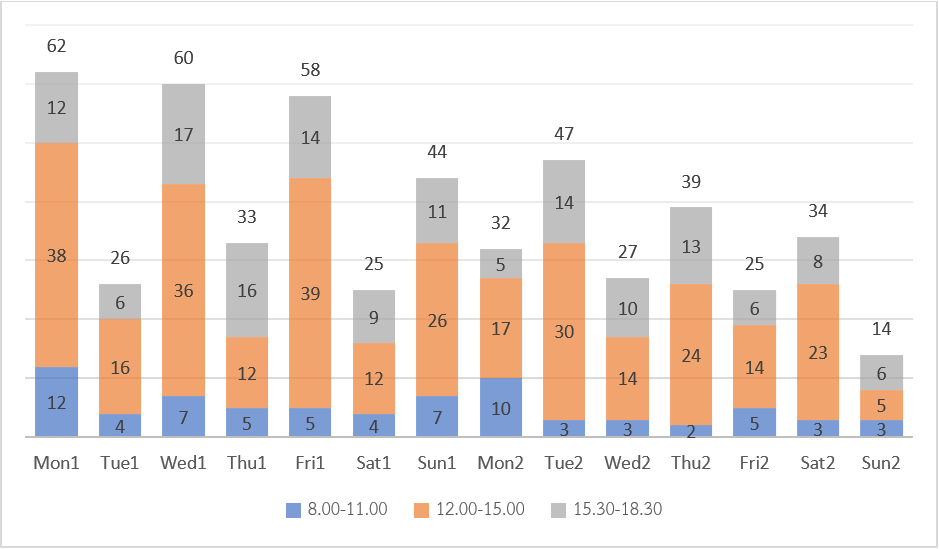
\includegraphics[width=\linewidth]{images/bar_chart_for_final_exam_slot.png}
  \end{center}
  \caption[Poem]{ความต้องการในสอบของผู้ตอบแบบสอบถามในแต่ละช่วงเวลา}
  \label{fig:time_slot}     
\end{figure}
\begin{enumerate}
  \item สัปดาห์ที่หนึ่ง เวลา 12.00-15.00น. วันศุกร์ 
  \item สัปดาห์ที่หนึ่ง เวลา 12.00-15.00น. วันจันทร์
  \item สัปดาห์ที่หนึ่ง เวลา 12.00-15.00น. วันพุธ
  \item สัปดาห์ที่สอง เวลา 12.00-15.00น. วันอังคาร
  \item สัปดาห์ที่หนึ่ง เวลา 12.00-15.00น. วันอาทิตย์
  \item สัปดาห์ที่สอง เวลา 12.00-15.00น. วันพฤหัสบดี
  \item สัปดาห์ที่สอง เวลา 12.00-15.00น. วันเสาร์
\end{enumerate}

ซึ่งจากกราฟ \ref{fig:time_slot} ยังสามารถสรุปได้ว่าผู้ทำแบบสอบถามส่วนใหญ่ต้องการที่จะสอบหนึ่งวันเว้นหนึ่งวันเพื่อที่จะได้มีเวลาในการอ่านหนังสือเตรียมสอบสำหรับวิชาในวันถัดไปมากกว่าการสอบติดกัน 
เรายังสามารถบอกเพิ่มเติมได้อีกว่าผู้ทำแบบสอบถามส่วนใหญ่ต้องการสอบในช่วงสัปดาห์แรกของช่วงการสอบมากกว่าช่วงสัปดาห์ที่สองเพื่อที่จะได้มีเวลาพักผ่อนหรือกลับบ้าน หลังจากที่สอบเสร็จแล้ว

\section{โครงสร้างและการทำงานของโปรแกรม}
\subsection{ข้อมูลที่จำเป็นสำหรับการพัฒนาโปรแกรม}
ข้อมูลนำเข้าของโปรแกรมจะเป็นไฟล์ text จำนวน 3 ไฟล์
\begin{itemize}
  \item ไฟล์ที่หนึ่ง ประกอบไปด้วย รหัสวิชา และ จำนวนนักศึกษาที่ลงทะเบียนในวิชานั้น ซึ่งจะถูกนำไปใช้ในการจัดลำดับความสำคัญของวิชา
  เพื่อให้วิชาที่มีนักศึกษาลงทะเบียนเป็นจำนวนมากถูกนำไปจัดในตารางสอบก่อน
  \item ไฟล์ที่สอง ประกอบไปด้วย รหัสวิชาของสองวิชาที่มีนักศึกษาอย่างน้อย 1 คน ลงทะเบียนทั้งสองวิชา และ จำนวนนักศึกษาที่ลงทะเบียนในคู่วิชานั้น ๆ 
  ใช้เพื่อเป็นตัวบ่งชี้ว่าสองวิชาที่ว่ามานี้จะต้องไม่ถูกจัดให้อยู่ในช่วงเวลาสอบเดียวกัน
  \item ไฟล์ที่สาม ประกอบไปด้วย รหัสวิชา และ จำนวนรายวิชาอื่น ๆ ที่มีนักศึกษาลงทะเบียนคู่กับรายวิชานี้
\end{itemize}

ข้อมูลผลลัพธ์ของโปรแกรมจะเป็นไฟล์ csv ที่ระบุตารางสอบรวม โดยระบุเป็นรายวิชาคู่กับวันและเวลาที่สอบของรายวิชานั้น ๆ
ส่วนสำหรับตารางสอบของนักศึกษารายบุคคลนั้นจะนำตารางสอบรวมนี้ไปประมวลผลอีกครั้งเพื่อระบุวันเวลาที่สอบของแต่ละรายวิชาที่นักศึกษาคนนั้น ๆ ลงทะเบียน




